\documentclass[conference]{IEEEtran}
\usepackage[utf8]{inputenc}
\usepackage{cite}
\usepackage{tabularx} % Required for the table
\usepackage{array}    % Required for custom column types
\usepackage{longtable}
\usepackage{booktabs}
\usepackage{adjustbox} % To allow scaling of tables
\usepackage{caption}
\usepackage{stfloats}
\usepackage{authblk}
\usepackage{algorithm}      % For algorithm environment
\usepackage{algpseudocode}  % For algorithmicx commands
\usepackage{amsmath}
\usepackage{float}



\begin{document}

\title{Power, Area and Thermal Prediction in 3D Network-on-Chip using Machine Learning}

\author{Abhijith C, Anand M K \\

Department of Computer Science and Engineering \\ 
	National Institute of Technology Karnataka (NITK) \\ 
	Surathkal, India\\
Email: \{abhijithc.242cs003, anandmk.242cs008\}@nitk.edu.in}


\maketitle

\section{Proposed Methodology}

Machine learning (ML) algorithms are widely used in various real-time predictions. The Power, Area, and Temperature (PAT) prediction of Network-on-Chip can also leverage the ability of machine learning models. Most existing studies focus on power, area, or thermal analysis independently. Frameworks involving simultaneous analysis of all three parameters are rare in current research. This work proposes a hybrid model that combines ML and DL algorithms. The ML component of the hybrid model uses algorithms such as linear regression and decision trees to predict area and power, which have a linear relationship with NoC parameters. The DL component of the model uses convolutional neural networks (CNNs) that learn complex non-linear relationships in NoC to predict temperature. The algorithms can predict PAT values for unseen input NoC configuration based on their learning. The prediction of both models is combined to produce a single output in the hybrid model.

\subsection{Dataset Creation}

The dataset generation process for power, area, and thermal prediction in NoC systems involves using different parameters specified in Table \ref{tab:noc_params} to generate different configurations for a NoC system. The different NoC parameters include topology, routing algorithm, network size, traffic pattern, buffer size, packet size, and packet injection rates (PIR). The dataset is created by changing the value of the parameters to generate different configurations for an NOC system.

The dataset creation is described in Algorithms 1 and 2. Step 1 involves generating different configurations of a NoC system by looping through different parameter values. Step 2 involves using a PAT-maxim simulator to simulate the different configurations generated in Step 1 and collecting output metrics, such as Average Power, Total Area, Average Temperature, etc., for each configuration. Step 3 involves storing the output metrics along with the configurations of the NoC system into a file such as a CSV file. This file will then be used to train the ML and DL models.


\begin{table}[h!]
\centering
\begin{adjustbox}{max width=\textwidth}
\begin{tabular}{|c|c|}
\hline
\textbf{NoC Parameter} & \textbf{Parameter Values} \\
\hline
\textbf{Topology} & 3D Mesh Topology \\
\hline
\textbf{Routing Algorithm} & 
\begin{tabular}[c]{@{}c@{}}
XYZ Routing, \\
OE\_3D (Odd-Even 3D Routing), \\
Full Adaptive Routing
\end{tabular} \\
\hline
\textbf{Network Size} & 
\begin{tabular}[c]{@{}c@{}}
\text{dimX: 2 to 16}, \\ 
\text{dimY: 2 to 16}, \\ 
\text{dimZ: 2}
\end{tabular} \\
\hline
\textbf{Traffic Pattern} & Random \\
\hline
\textbf{Buffer Size} & 4 \\
\hline
\textbf{Packet Size} & 4  \\
\hline
\textbf{Packet Injection Rate (PIR)} & 
\begin{tabular}[c]{@{}c@{}}
0.01, 0.02, 0.03, \ldots, 0.1
\end{tabular} \\
\hline
\textbf{Sample Period} & 200000 \\
\hline
\end{tabular}
\end{adjustbox}
\caption{NoC Parameters and Values}
\label{tab:noc_params}
\end{table}

\begin{algorithm}[H]
\caption{Generate NoC Configurations}
\label{algo_step1}
\begin{algorithmic}[1]
    \State \textbf{Input:} Set of NoC parameters:
        \begin{itemize}
            \item \textbf{Topology}: 3D Mesh Topology
            \item \textbf{Routing Algorithms}: 
                \begin{itemize}
                    \item XYZ Routing
                    \item OE\_3D (Odd-Even 3D Routing)
                    \item Full Adaptive Routing
                \end{itemize}
            \item \textbf{Network Size}: 
                \begin{itemize}
                    \item dimX: 2 to 16
                    \item dimY: 2 to 16
                    \item dimZ: 2
                \end{itemize}
            \item \textbf{Traffic Pattern}: Random
            \item \textbf{Buffer Size}: 4 
            \item \textbf{Packet Size}: 4
            \item \textbf{Packet Injection Rate (PIR)}: 
                \begin{itemize}
                    \item 0.01, 0.02, 0.03, 0.04, 0.05, 0.06, 0.07, 0.08, 0.09, 0.1
                \end{itemize}
            \item \textbf{Sample Period}: 200,000 cycles
        \end{itemize}
        
    \State \textbf{Step 1: Generate Configurations}
    \For {dimX from 2 to 16}
        \For {dimY from 2 to 16}
            \For {each routing algorithm in Routing Algorithms}
                \For {each PIR in Packet Injection Rate}
                    \State Create a configuration with parameters: 
                        \{topology, dimX, dimY, dimZ, traffic pattern, PIR, buffer size, packet size, sample period, routing algorithm\}
                    \State Store the configuration in a list
                \EndFor
            \EndFor
        \EndFor
    \EndFor
\end{algorithmic}
\end{algorithm}

\begin{algorithm}[H]
\caption{Simulate Configurations and Save Dataset (Continued)}
\label{algo_step2_3}
\begin{algorithmic}[1]
    \State \textbf{Step 2: Simulate and Gather Metrics}
    \For {each configuration in the list}
        \State Run the Noxim simulation with the current configuration
        \State Capture metrics:
            \begin{itemize}
                \item Total Area (um\(^2\))
                \item Avg Power (J/cycle)
                \item Avg Cores Power (J/cycle)
                \item Avg Routers Power (J/cycle)
                \item Avg Power per Router (J/cycle)
                \item Layer Area (um\(^2\))
                \item Area per Core (um\(^2\))
                \item Steady state temperature - L0
                \item Steady state temperature - L1
                \item Router Average Temperature - L0
                \item Router Average Temperature - L1
                \item Core Average Temperature - L0
                \item Core Average Temperature - L1
                \item Memory Average Temperature - L0
                \item Memory Average Temperature - L1
            \end{itemize}
    \EndFor
    
    \State \textbf{Step 3: Save Dataset}
    \State Save the dataset with all configurations and metrics to a file (e.g., CSV)
\end{algorithmic}
\end{algorithm}




\subsection{Linear Regression}

Linear regression is an ML algorithm that is used for predictions involving numerics. It learns the relationship between dependent (output) and independent (input) variables by fitting a linear equation. The equation is represented as:

\[
Y = \beta_0 + \beta_1 X_1 + \beta_2 X_2 + \dots + \beta_n X_n + \epsilon
\]

where \( Y \) is the predicted output, \( X_1, X_2, \dots, X_n \) are the input, \( \beta_0 \) is the intercept, \( \beta_1, \beta_2, \dots, \beta_n \) are the coefficients, and \( \epsilon \) is the error term. The coefficients of the equation are learned using Mean Squared Error (MSE), a loss function. In power, area, and thermal (PAT) prediction for networks-on-chip (NoC), linear regression can predict these metrics based on input parameters such as topology size, packet injection rate, etc. However, linear regression learns only the input-output linear relationships. Therefore, methods such as decision trees are needed to learn the non-linear and complex relationships present in NoC systems.

\subsection{Decision Trees}

Decision trees are powerful ML algorithms used for regression and classification tasks. These algorithms split the training dataset based on the most significant feature that separates the data most precisely. The internal nodes of the decision tree define the decision on an input feature, and the leaf node represents the predicted output value. Decision trees can find complex input-output relationships as they are non-parametric. In power, area, and thermal prediction in NoC systems, complex relationships between NoC parameters can be learned using these algorithms. Decision trees help researchers understand which features impact the outputs the most by providing a visual structure. However, these algorithms can result in an overfitted model with increased generalization error. Generalization error can be reduced using techniques like pruning, making these algorithms perform well in large-scale NoC systems.

\subsection{Convolutional Neural Networks (CNNs)}

CNNs are used for tasks such as Image processing and Object detection. They apply filters using convolutional layers to extract features from the input dataset, making CNN the best algorithm for learning data structured in grid-like topologies, such as NoC systems. In power, area, and thermal prediction in the NoC system, CNNs can be used to understand non-linear relationships required for temperature prediction. CNNs can learn complex patterns in NoC designs that may not be possible for simpler algorithms like linear regression and decision trees. They work well with large datasets.



\subsection{Design of Proposed Method}
Algorithm 3 describes the flow of the proposed method. Step One involves dataset generation using the PAT-Noxim simulator, as described in Algorithms 1 and 2. The dataset is normalized to ensure that all the parameters equally contribute to the ML prediction. The duplicate data is removed to ensure the proposed model is trained on different data. The dataset is split into training (70\%), testing (15\%), and validation (15\%).

The proposed hybrid model includes ML components for Power and Area prediction and DL components for Temperature prediction. The training of the linear regression model minimizes the MSE between the predicted and actual values of power and area. 

\[
MSE = \frac{1}{n} \sum_{i=1}^{n} \left( Y_i - \hat{Y_i} \right)^2
\]

Where:
\begin{itemize}
    \item \( Y_i \): Actual output
    \item \( \hat{Y_i} \): Predicted output
    \item \( n \): Number of samples
\end{itemize}
The ability of the model to predict power and area on unseen NoC configurations are evaluated using the MSE.
The dataset is also trained on a decision tree algorithm to predict the power and area. This training phase involves splitting the dataset based on the most significant feature that separates the data most precisely. The MSE is used to calculate the ability of the model to predict accurately. 

The CNN model is designed to train the dataset for temperature prediction. The architecture consists of the following layers:

\begin{itemize}
	\item \textbf{Input Layer}: Accepts the input parameters.
	
	\item \textbf{Convolutional Layer 1}: Applies a set of convolutional operations to extract features from input. ReLU is used as an activation function.
	\begin{itemize}
		\item ReLU returns the maximum of 0, and the input value introduces non-linearity in the model. It can be represented as:
		\[
		f(x) = \max(0, x)
		\]
	\end{itemize}
	
	\item \textbf{Max-Pooling Layer}: Reduces the size of the feature map without losing extracted information.  
	
	\item \textbf{Convolutional Layer 2}: Extracts more features from the pooled feature map.
	
	\item \textbf{Flattening Layer}: Converts the feature map to a single-dimensional vector.
	
	\item \textbf{Fully Connected Layer}: Aggregates the learned features.
	
	\item \textbf{Output Layer}: Outputs the predicted thermal value with a linear activation function. The linear function output is the same as the input. It can be represented as:
	\[
	f(x) = x
	\]
\end{itemize}
The predicted power area and temperature are combined, and the model is tested using a test dataset. The flowchart of the proposed method is given in Figure 1.

\begin{algorithm}[H] % Forces it to stay here, potentially at the top of the column
\caption{Algorithm for Proposed Framework}\label{alg:pat_prediction}
\begin{algorithmic}[1]
    \State \textbf{Input:} Set of NoC parameters: Topology, Traffic Pattern, PIR (X, Y, Z), Buffer Size, Packet Size, Sample Period
    \State \textbf{Output:} Predicted values of Power, Area, and Temperature
    
    \State \textbf{Step 1: Dataset Creation}
    \State Create dataset using simulation tool (PAT Noxim) based on input NoC parameters
    \State Extract Power, Area, and Temperature as output labels
    
    \State \textbf{Step 2: Data Preprocessing}
    \State Normalize or scale the dataset
    
    \State \textbf{Step 3: Train-Test Split}
    \State Split the dataset into Training, Validation, and Test sets (e.g., 70\% training, 15\% validation, 15\% testing)
    
    \State \textbf{Step 4: Model Training}
    \State \textbf{ML Component:}
    \State Train a \textbf{Linear Regression} model for Power and Area prediction
    \State Train a \textbf{Decision Tree} model for Power and Area prediction
    
    \State \textbf{DL Component:}
    \State Train a \textbf{CNN} for Temperature prediction
    
    \State \textbf{Step 5: Model Evaluation}
    \State Use validation data to evaluate both models
    
    \State \textbf{Step 6: Combine Predictions}
    \State Combine the outputs from the ML and DL models for final Power, Area, and Temperature predictions
    
    \State \textbf{Step 7: Testing and Final Prediction}
    \State Test the combined model on the test set and make the final prediction
    
    \State \textbf{End}
\end{algorithmic}
\end{algorithm}

\begin{figure}[H]  % Begin the figure environment
    \centering
    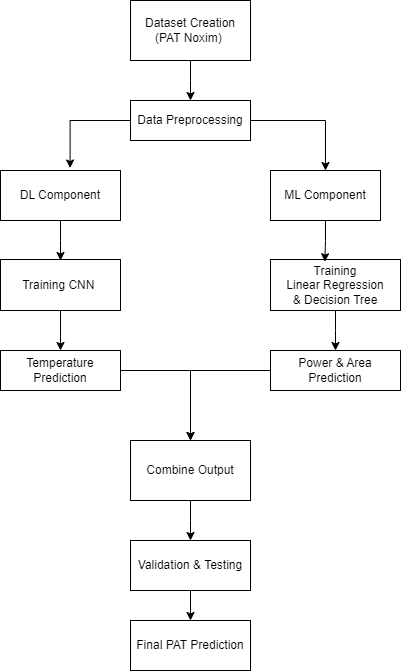
\includegraphics[width=0.8\linewidth]{Proposed.png}  % Specify the path to your image
    \caption{Illustration of the Proposed Framework}  % Add a caption for the image
    \label{fig:proposed_framework}  % Add a label for referencing the image
\end{figure}


\end{document}
